\documentclass[12pt]{article}
\usepackage{geometry}
\usepackage{amsmath}
\usepackage{amssymb}
\usepackage{enumitem}
\usepackage{fancyhdr}
\usepackage{tikz}
\usepackage{color}
\usepackage{xspace}
\usepackage{thumbpdf}
\usepackage{listings}
\usepackage{verbatim}
\usepackage{hyperref}
\usepackage{booktabs}
\usepackage{colortbl}
\usetikzlibrary{trees}
\usetikzlibrary{shapes,arrows}
\pagestyle{fancy}

\newcommand{\xref}[1]{\S\ref{#1}}
\definecolor{darkred}{rgb}{0.7,0,0}
\definecolor{darkgreen}{rgb}{0,0.5,0}
\hypersetup{colorlinks=true,
	linkcolor=darkred,
	citecolor=darkgreen}

\lstset{
	basicstyle=\ttfamily,
	mathescape
}

\lstdefinestyle{customc}{
	belowcaptionskip=1\baselineskip,
	breaklines=true,
	% xleftmargin=20pt,
	language=matlab,
	% frame=L,
	escapeinside={@}{@},
	showstringspaces=false,
	basicstyle=\small\ttfamily,
	keywordstyle=\bfseries\color{green!40!black},
	commentstyle=\itshape\color{purple!40!black},
	%identifierstyle=\color{blue},
	stringstyle=\color{orange},
	% directivestyle=\color{brown},
	%numbers=left,
	%numberstyle=\tiny\color{gray}
}

\lstdefinestyle{customctable}{
	aboveskip=-\medskipamount,
	belowskip=-\medskipamount,
	language=C,
	escapeinside={@}{@},
	showstringspaces=false,
	basicstyle=\scriptsize\ttfamily,
	keywordstyle=\bfseries\color{green!40!black},
	commentstyle=\itshape\color{purple!40!black},
	%identifierstyle=\color{blue},
	stringstyle=\color{orange},
	directivestyle=\color{brown},
}

\textheight=8.5in

\newcommand{\hongzi}[1]{{{\color{red}(HM: #1)}}}

\lhead{6.854 Pset 5}
\chead{Hongzi Mao  \: \footnotesize{collaborators:} Calvin Lee, Linus Hamilton}
\rhead{Oct 12, 2016}

\begin{document}
	
\section*{Problem 1}
\paragraph{(a)}
We are given the table and we need to check if the set of disclosed elements are feasible. We construct a graph in Figure \ref{fig:1-a}. First, we create source $s$, sink $t$ and a layer of nodes for each row sum $r_1, r_2, ..., r_p$ and each column sum $c_1, c_2, ..., c_q$. Then, for each row $i$ we compute $r_i' = r_i - \sum_{j \in Y_i} d_{ij}$, where $Y_i$ contains all disclosed elements in $Y$ and row $i$. Similarly we deduct elements in $Y$ from column sums. Next, connect $s$ with each $r_i$ with capacity $r_i'$, and connect each $c_i$ with $t$ with capacity $c_i'$. Finally, for each element $d_{ij}$ \emph{not} in $Y$, connect $r_i$ with $c_j$ with capacity $\infty$.

\begin{figure}[h!]
	\centering
	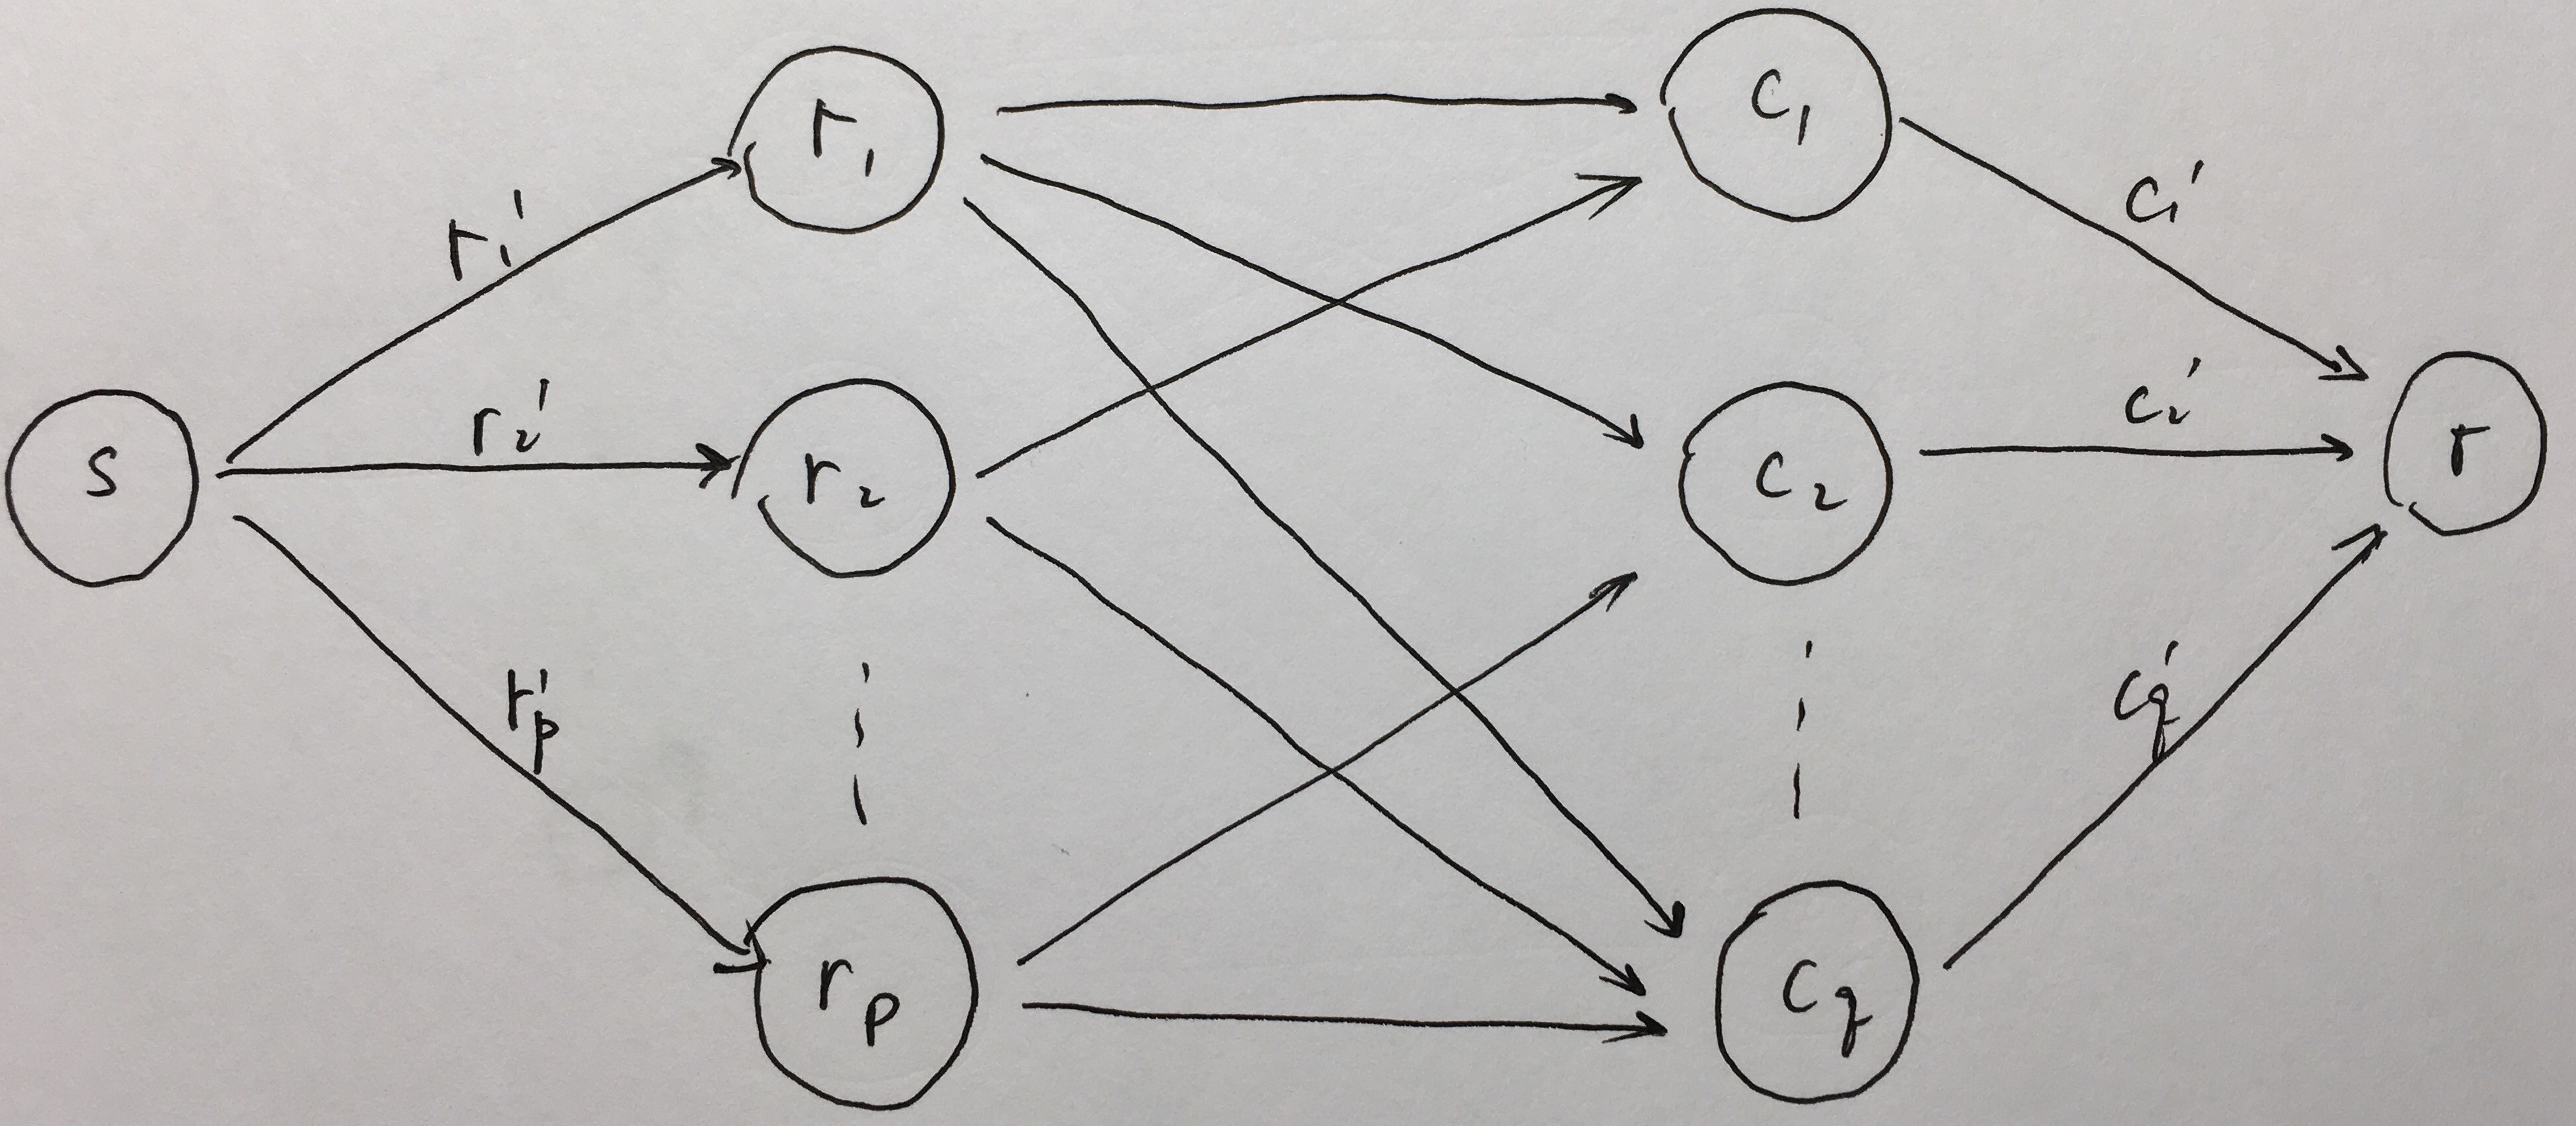
\includegraphics[width=0.7\textwidth]{1-a.jpg}
	\caption{Illustration of graph setup. Notice that in this example, $d_{22}$ and $d_{p1}$ is in $Y$ as the edge between $r_2, c_2$ and the edge between $r_p, c_1$ are disconnected.}
	\label{fig:1-a}
\end{figure}

Now we run a max-flow algorithm on this graph. If the maximum flow equals to $\sum_{i=1}^{p} r_i'=\sum_{i=1}^{q} c_i'$, then there is some set of cell values that produces the disclosed values. This is because we can set the flow value between row node and column node to be the cell value. The flow conservation property on nodes guarantees the sums on the rows and columns all check out. The max flow value makes sure sums on the rows and columns equal to the disclosed values. Moreover, if there exists a \emph{known} set of cell values, this flow based algorithm should return positive for the feasibility. This is because we can plug in the known values in the edge and saturate the edges from source and edges to the sink, therefore being maximum. If the algorithm returns negative, it means the max flow returns a smaller value, which is a contradiction. 

Constructing $p$ row nodes and edges to $s$ take $O(p)$, similarly column nodes take $O(q)$. The connection between row and column nodes take $O(pq)$. Hence total construction time takes $O(pq)$. 

\paragraph{(b)}
With the max flow $f$ and the edge $e(u, v)$, we look into the residual graph $G_f$. The goal is to find a loop including $u$ and $v$ such that we can push flow through, therefore make a different flow on edge $e$, but \emph{still} preserves the max flow. To do this, we $\emph{disconnect}$ the edge between $u$ and $v$ on residual graph, and then use BFS to find a path from $v$ to $u$. If such a path exists, with the edge $e(u,v)$ connecting back, we know a flow can be pushed on the loop, first from $u$ to $v$ and then through some other paths back to $u$. Also, we can apply similar technique for the other direction to create loop from $v$ to $u$ then through some paths back to $v$. Both actions can affect flow on edge $e$ but preserve total max flow value. 

If these two BFS searches of loop returns no valid loop, we know the flow of edge $e$ is \emph{unique} in max flow. Because otherwise we could have subtract two max flow from each other and create a circulation for edge $e$, which is a contradiction. 

The checking takes $O(2(m+n)) = O(m)$ since the two direction BFS at most go through all edges and nodes twice.

\paragraph{(c)} The node $d_{ij}$ on table is \emph{unprotected} if its value is \emph{uniquely} determined. Therefore, with a feasible max flow on Figure \ref{fig:1-a}. we can examine each $d_{ij}$ by checking if the flow on edge $e(i,j)$ can be altered while preserving the max flow in the graph. If it can be altered, it means there can be different possible value of $d_{ij}$ that results in same disclosed set of values, which therefore means $d_{ij}$ is protected. To do so, we use the algorithm in (b) on each edge $e(i,j)$. Notice that total number of edges on the graph is $O(pq)$ each checking can take $O(pq)$ time. Therefore the total checking time is $O(p^2q^2)$.

\pagebreak

\section*{Problem 2}
It is not necessary the min-cost max-flow in the graph. Consider the example graph in the following. For shortest augmenting path algorithm, it will first push flow on the path of length 4. Then, the path on top and the other path in the middle can not be used as part of the them is saturated. As a result, another flow takes the bottom path. The cost of this max flow is therefore $4+7=11$. The path it chooses is denoted by blue arrows in the graph. 

The blocking flow algorithm will pick the same paths. First, the `distance' between $s$ and $t$ is $4$ and it sends a flow to `block' it. After this step, only length $7$ path can be used. 
\begin{figure}[h!]
	\centering
	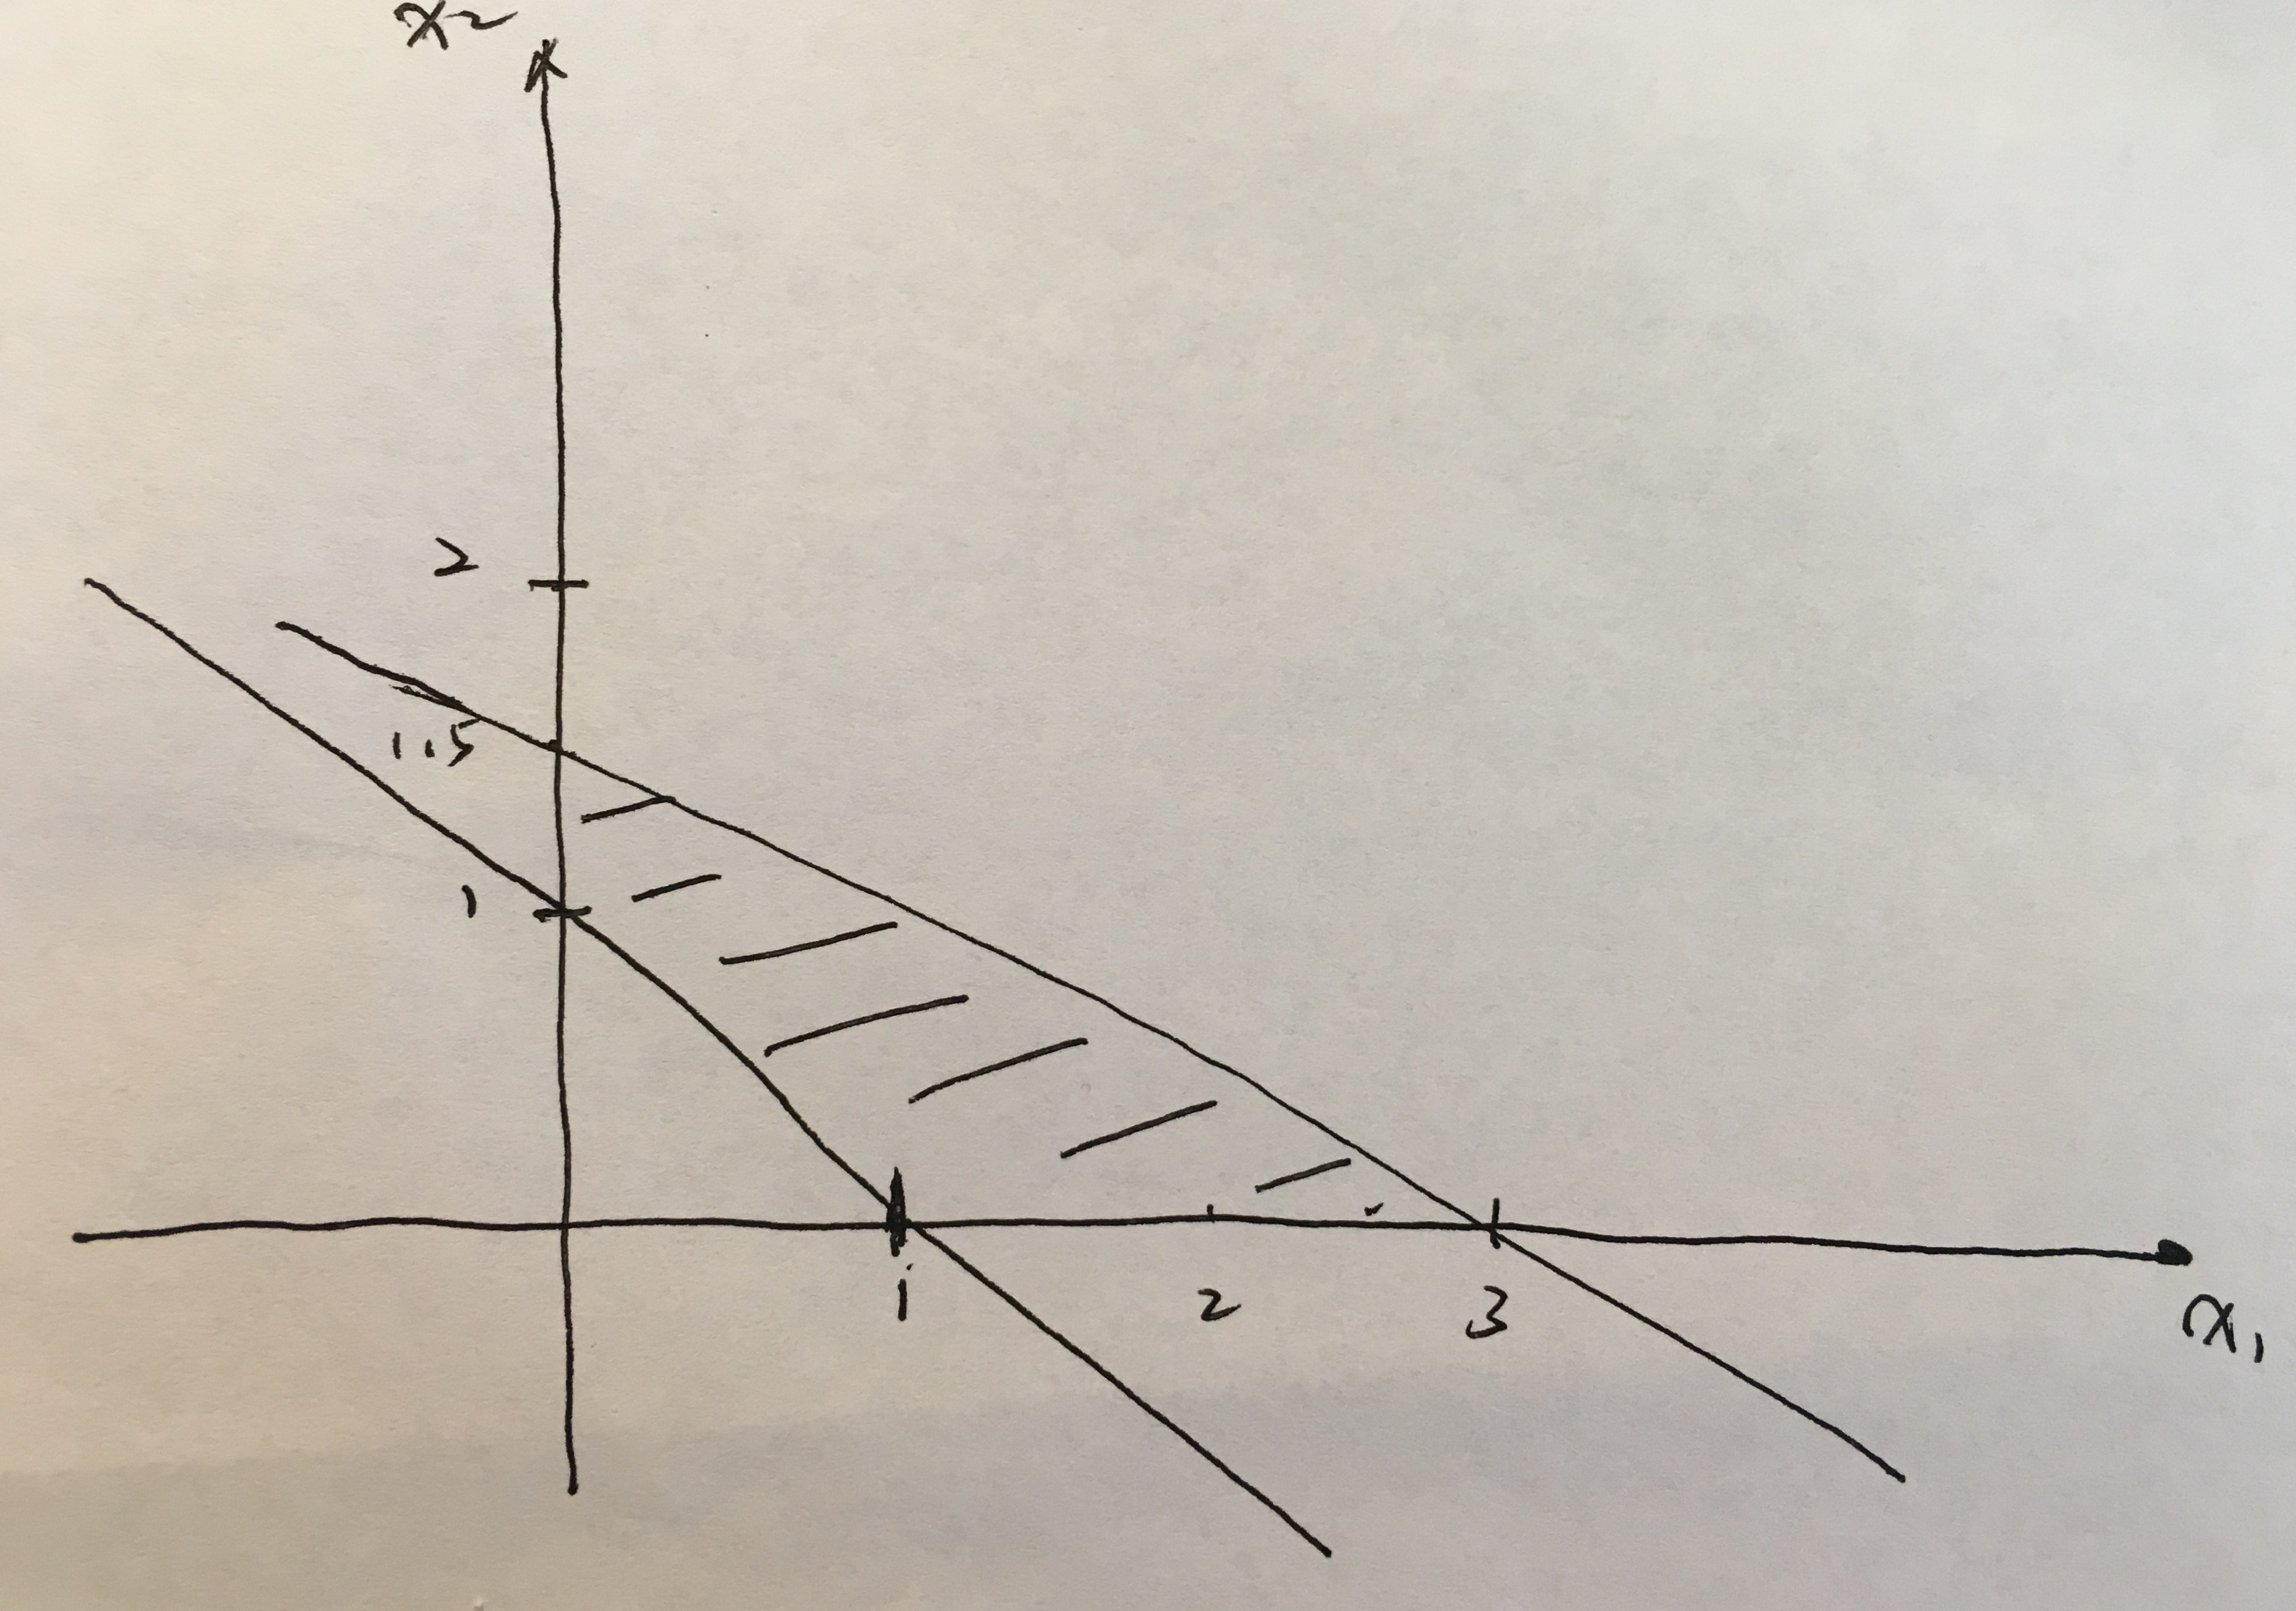
\includegraphics[width=0.7\textwidth]{2.jpg}
	\label{fig:2}
\end{figure}

However, the min-cost max flow is the to use the top path and the middle lower path, which give a smaller cost $5 + 5 = 10$. The min-cost max-flow is denoted by red arrows in the graph. Therefore, it is not necessary that shortest augmenting path algorithm or standard blocking flow algorithm returns the min-cost max-flow in the graph.

\pagebreak

\section*{Problem 3}
\paragraph{(a)} The problem can be fit into classic bipartite matching problem as in Figure \ref{fig:3-a}. We connect each student to a source node and each recitation to a sink node. Then, connect each student to the recitation that she is able to attend. Next, set the capacity to be 1 for all links. Finally, we run max flow algorithm atop this graph; if the max flow equals to the total number of student, then there is a feasible allocation of students to recitations. 

The max flow result can be student recitation allocation directly, therefore max flow being total number of students means feasible allocation exists. Also, if max flow is less, it means feasible allocation does not exist. Because otherwise we could have assign the flow based on the feasible allocation and break the max flow property. 

Although phrasing it as a max flow problem, we know this classic bipartite matching problem can be solved\footnote{E.g., Hopcroft–Karp algorithm.} in $O(m\sqrt{n})$. We now use another analysis to show that blocking flow based max flow algorithm on this problem can also achieve $O(m\sqrt{n})$. 

When invoking blocking flow algorithm, after $b$ blocking flow, the distance between $s$ and $t$ becomes $b$, the total number of residual flow is bounded\footnote{from Pset 4 problem 4 (a)} by $n/b$. In unit capacity graph, the flow paths are edge disjoint (one goes in, ones goes out), therefore, the total number of flow path is at most $n/b$. Therefore, it requires at most $n/b$ blocking flow to reach max flow. To minimize $b + n/b$, we set $b=\sqrt{n}$. Each blocking flow traverses at most $m$ nodes. Therefore, the max flow can be achieved in $O(m\sqrt{n})$ time.
\begin{figure}[h!]
	\centering
	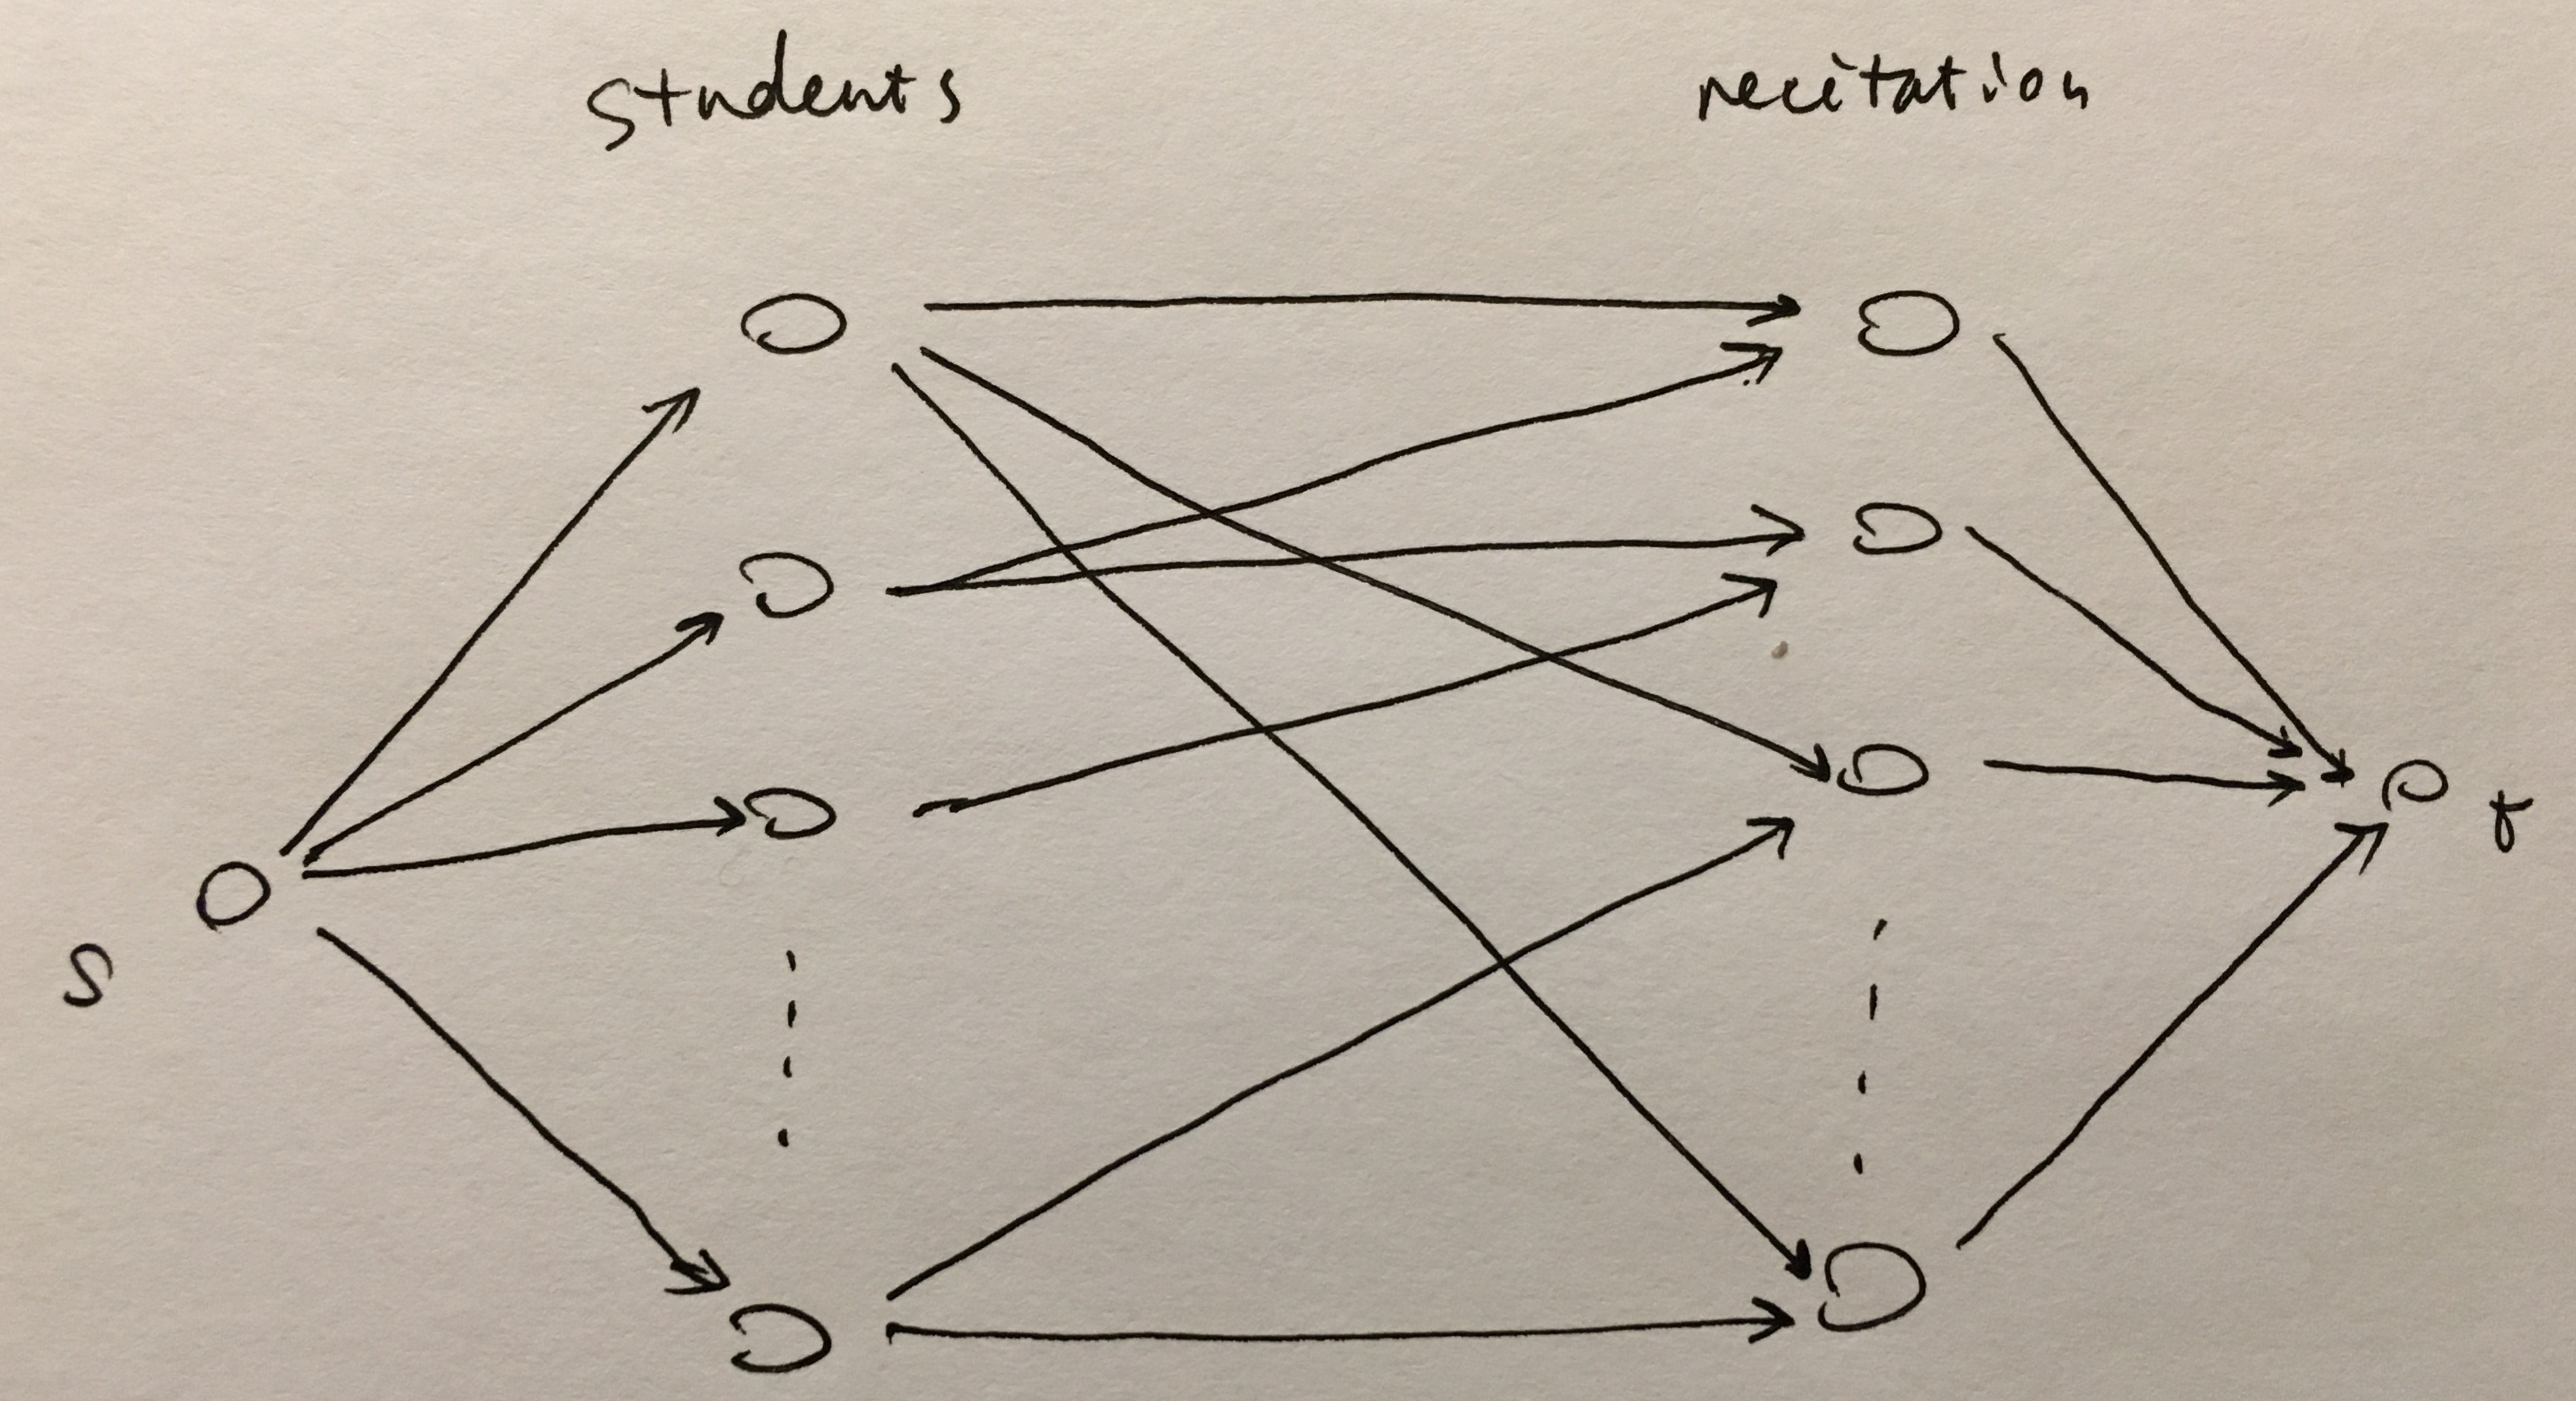
\includegraphics[width=0.7\textwidth]{3-a.jpg}
	\caption{Student-recitation matching problem as classic bipartite matching problem. Link a student to a recitation if the student can go to that recitation. As above, for example, the first student can go to first, third and last recitation. The capacity is $1$ for all links.}
	\label{fig:3-a}
\end{figure}
\paragraph{(b)} We modify the capacities of the links between recitation to sink $t$ to be $k$ instead of $1$ in (a). Then, we run max flow algorithm; if the max flow equals to the total number of student, then there is a feasible allocation of students to recitations. 

The correctness of the algorithm can be argued similarly as (a). The max flow result here can still be student recitation allocation directly, therefore max flow being total number of students means feasible allocation exists. Also, if the max flow is less, it means feasible allocation does not exist. Because otherwise we could have assign the flow based on the feasible allocation and break the max flow property. 
\paragraph{(c)} If we look closer into the argument in (a) we can find that $O(m\sqrt{n})$ bound still works when we augment the edge capacity in the final layer to be $k$. In (a), when the distance is $n/b$, the total number of flow path is still at most $n/b$. This is because when we account for the largest set of edge-disjoint paths, only the last hop changes its capacity to k, flow to any other node still obey edge disjoint property. In order words, the maximal collection of edge-disjoint admissible paths is `bottlenecked' on nodes on students layer, not the recitation layer. More precisely, for any link pointing to the nodes at student layer in residual graph, the flow can only goes to \emph{one} other link via the student node. Thus, edge-disjoint analysis on (a) still holds. Therefore, we can still set $b=\sqrt{n}$ and obtain $O(m\sqrt{n})$ as the time bound for total finding max-flow.

\pagebreak

\section*{Problem 4}
\paragraph{(a)} An example is shown in Figure \ref{fig:4-a}. The total flow value is 1 and it evenly is splitted into two flows of 0.5. Notice that the total cost on the upper two links is $0.4 + 0.4 = 0.8$, which is the same as the cost of the lower link. Therefore, the flow is a min-cost flow.
\begin{figure}[h!]
	\centering
	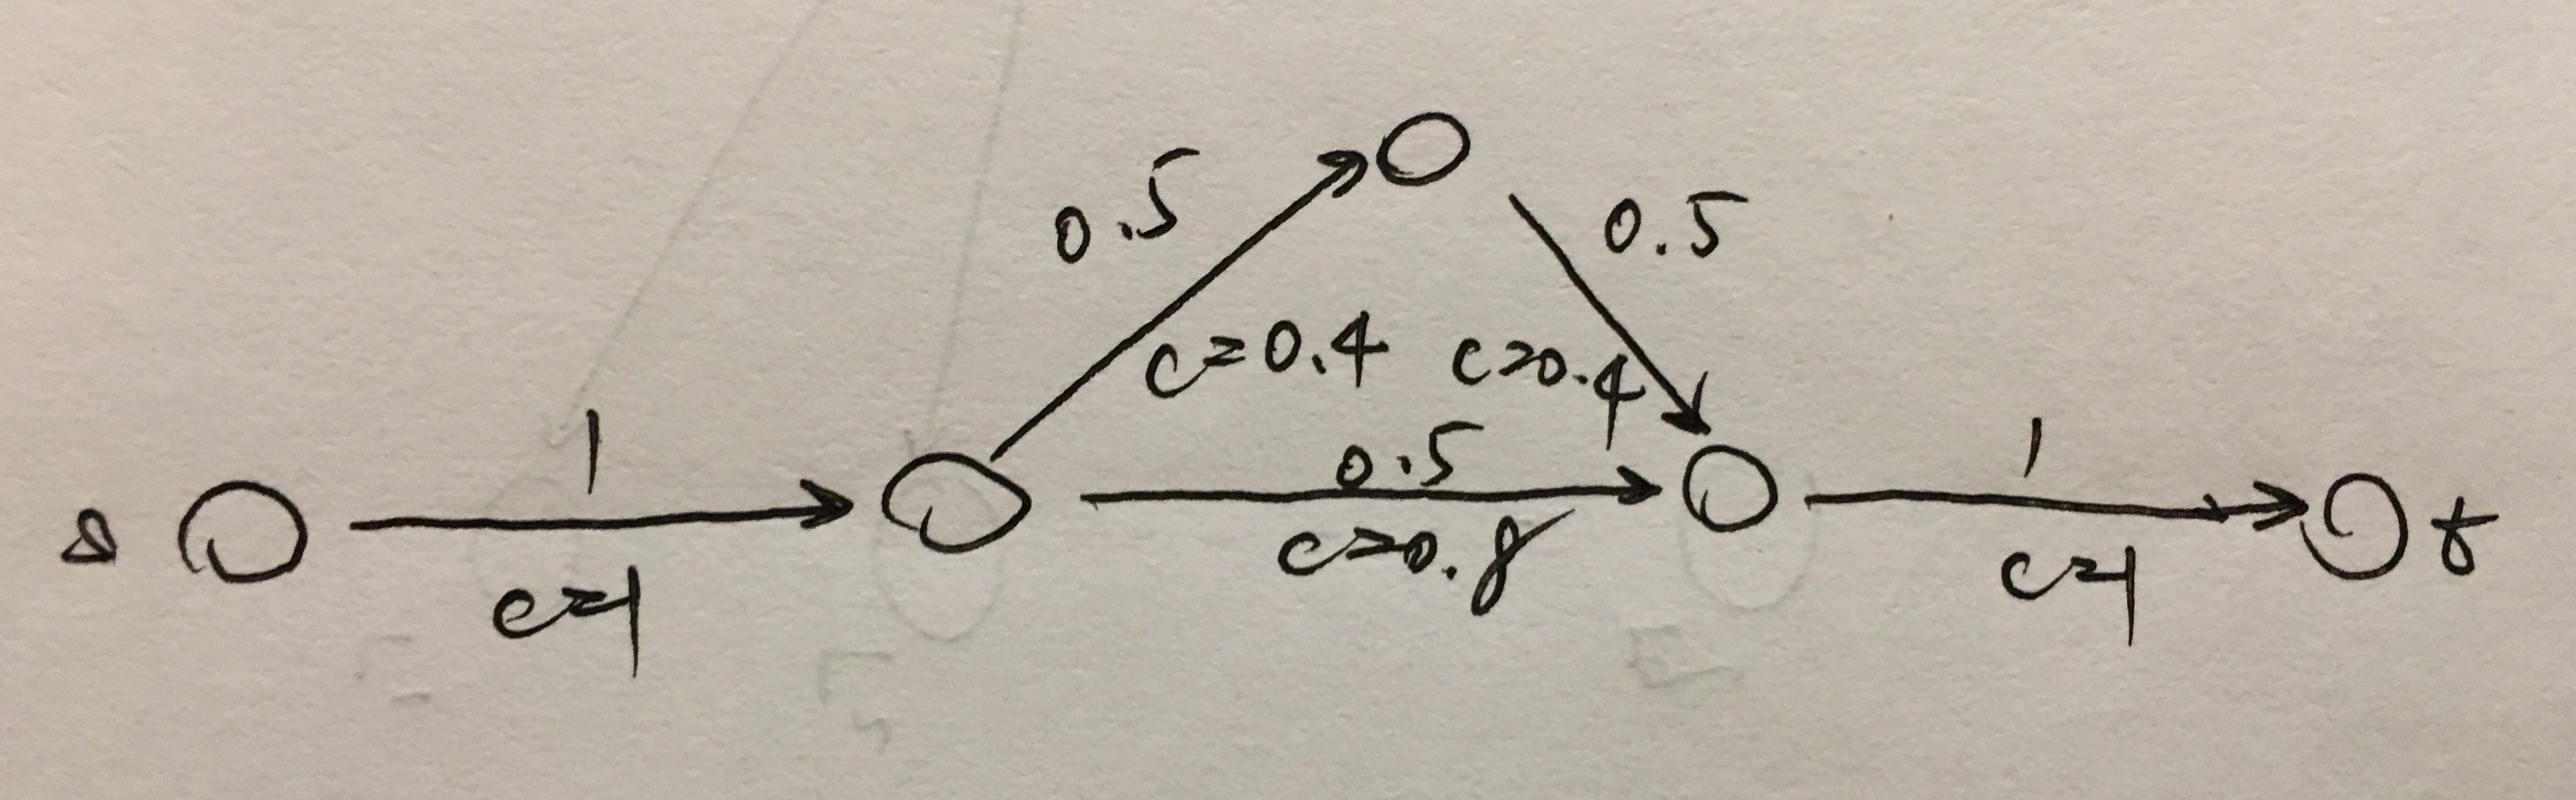
\includegraphics[width=0.7\textwidth]{4-a.jpg}
	\caption{An example of fractional min-cost flow. Flow is marked on the top of each link, and the cost in marked on the bottom. The capacities for all links are $1$.}
	\label{fig:4-a}
\end{figure}
\paragraph{(b)} In Figure \ref{fig:4-b}, we zoom in the triangle area of the residual graph of the example in Figure \ref{fig:4-a}. Notice that the backward links on the upper half have capacity $0.5$, where a flow of this value can be pushed and be pushed forward on the lower link, which has a residual capacity $0.5$ on the forward link, which causes a cycle of fractional capacity. 
\begin{figure}[h!]
	\centering
	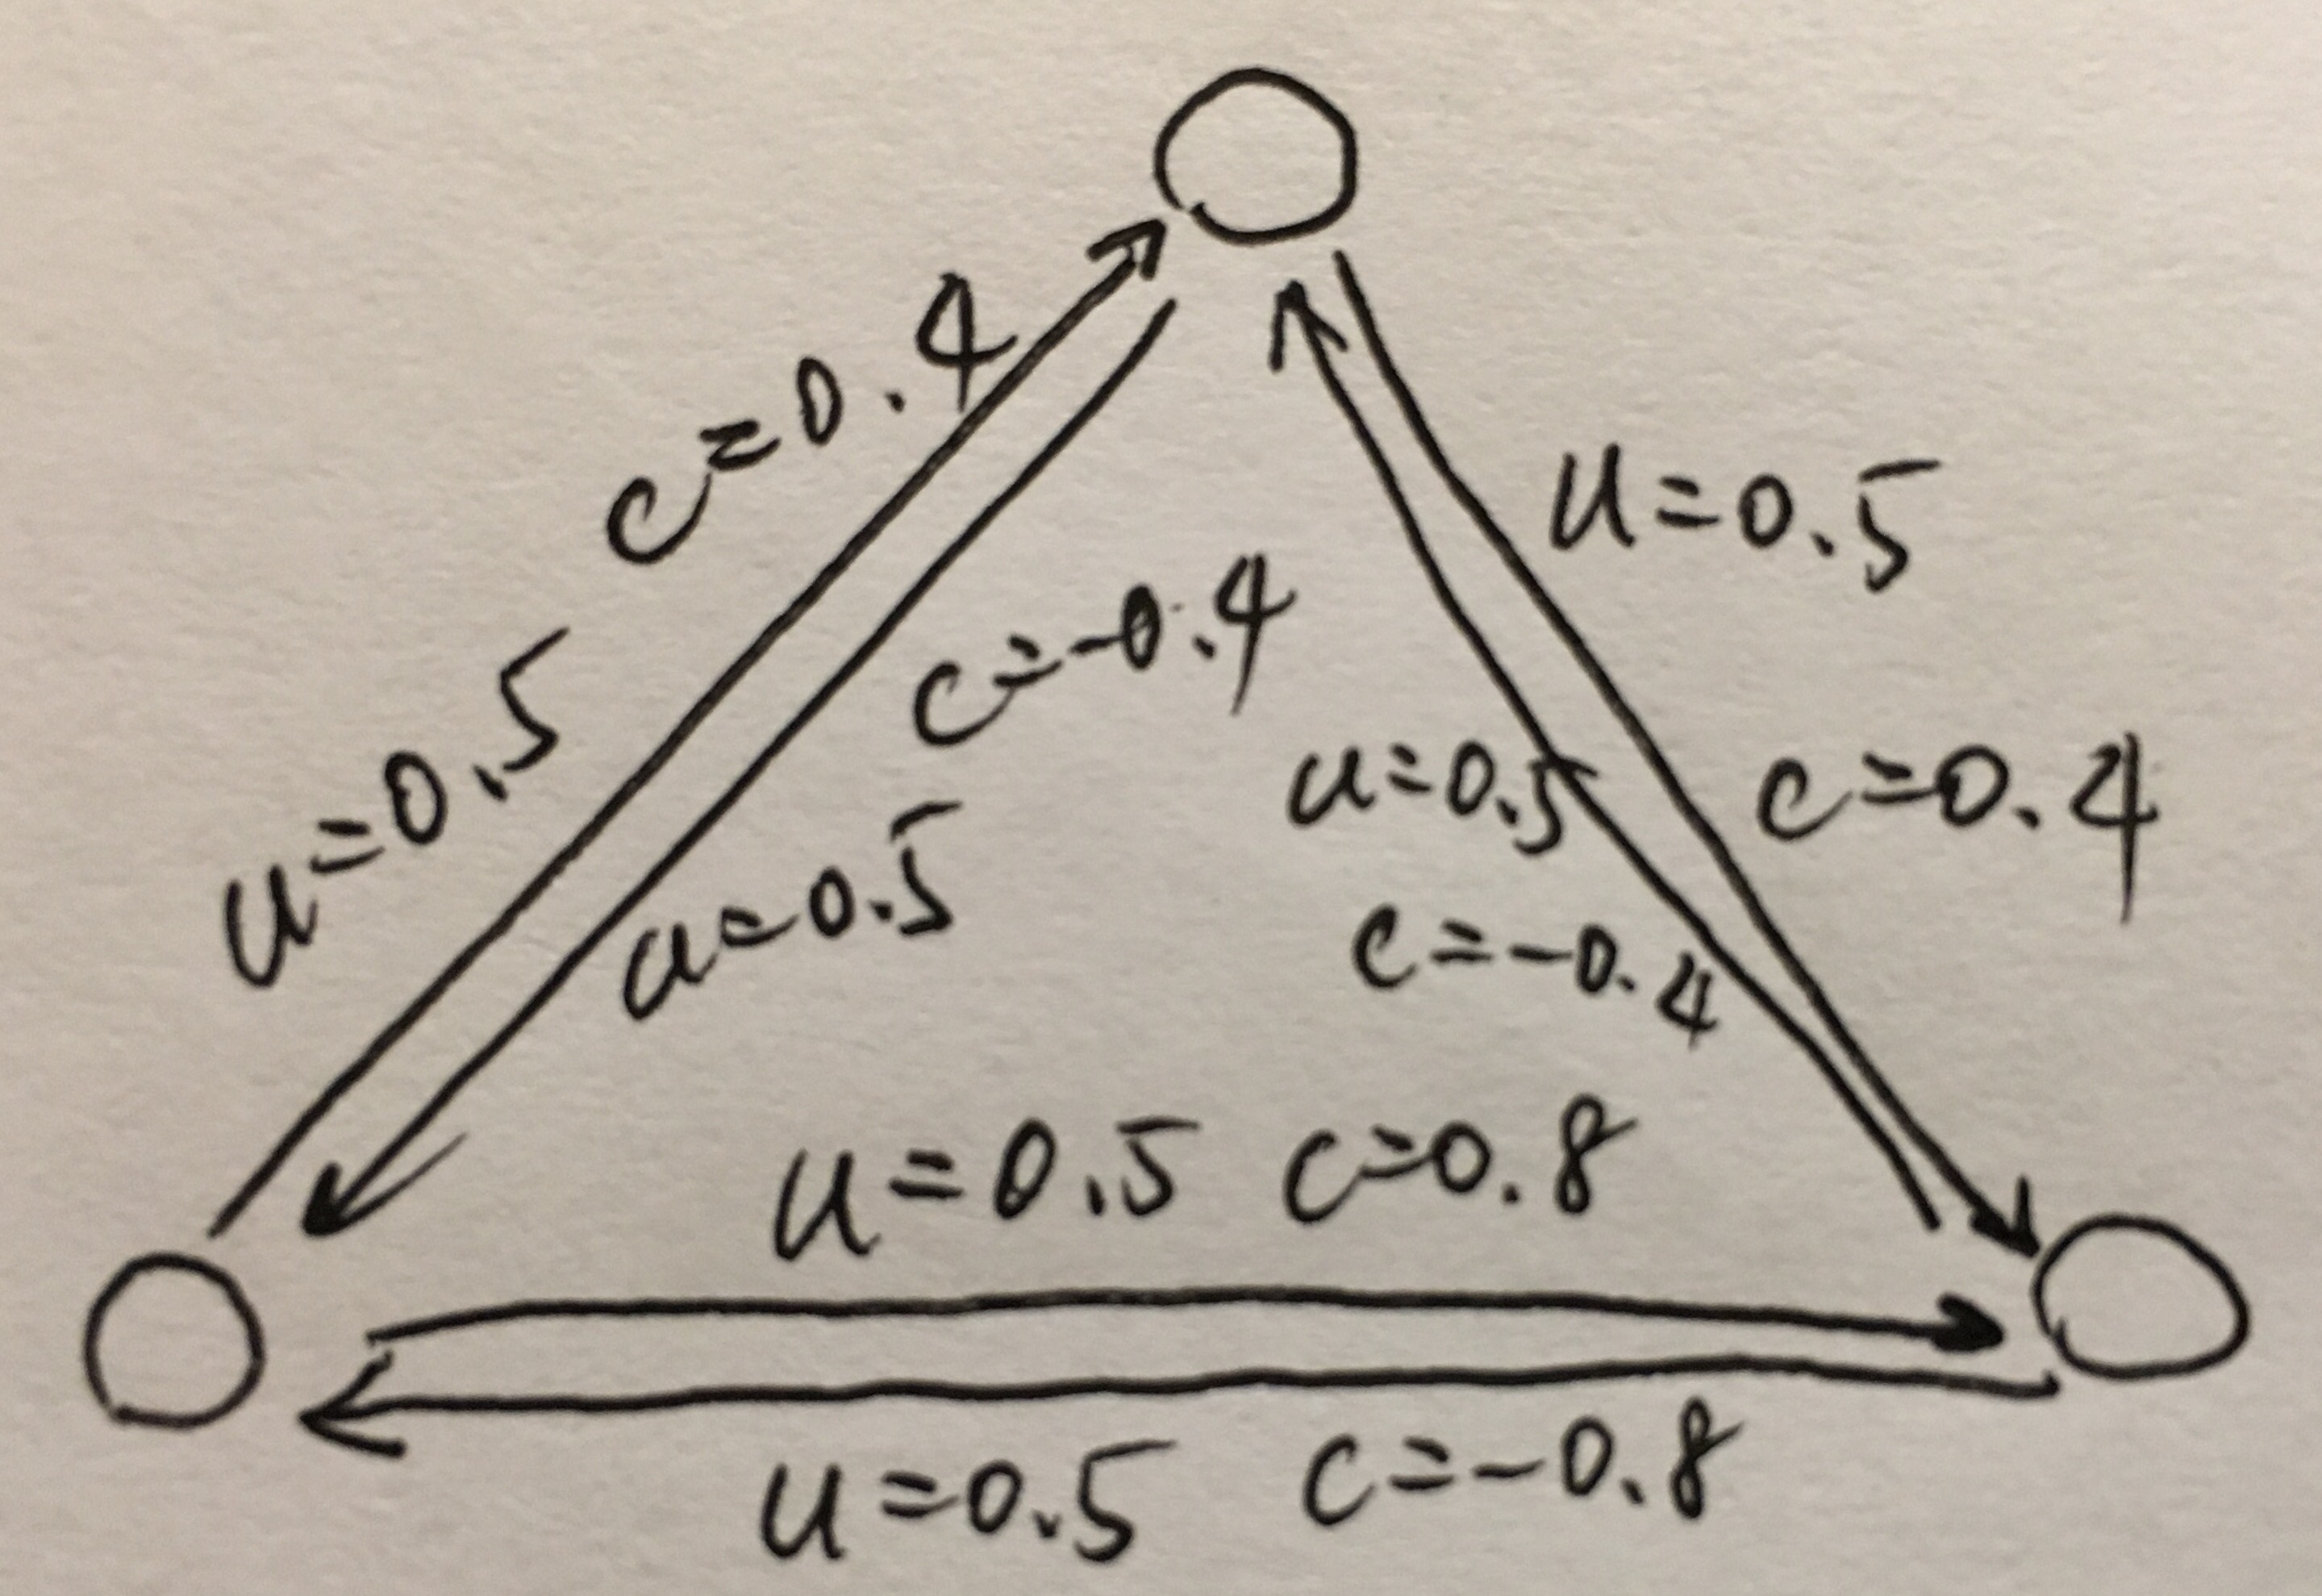
\includegraphics[width=0.4\textwidth]{4-b.jpg}
	\caption{Zoom in on the triangle part of the residual graph $G_f$ of Figure \ref{fig:4-a}. The capacity and cost of the links are marked accordingly.}
	\label{fig:4-b}
\end{figure}

In general, for any of such flow, the residual graph must contain a cycle of edges of fractional capacity. This is because, in the original graph, since the capacities are all integers there must be a `fork' at which the integer flow is splitted into multiple fractional flows. The cost on the forks towards $t$ should be all the same, otherwise we could have push flow on some certain path to get a smaller cost (this can be achieved because the capacities are all integers, fractional flow must leave some room free). Then in the residual graph, the paths the forks traverse through make a cycle with fractional capacity.
\paragraph{(c)} The total cost of this cycle is 0. On Figure \ref{fig:4-b}, notice that the cost of the backward links are $-0.4$ on the upper two links, which cancels the cost $0.8$ on the forward residual link in the lower part. 

In general, the total cost $0$ still holds. This is because of the following. (1) Assume on the cycle, the cost is smaller than $0$, then we could have push a flow through the cycle to obtain a smaller total cost while still maintaining the total flow value, which contradicts with the min-cost property. (2) If the cost is on the cycle is larger than $0$ and the flow into the cycle is integral (i.e., the example in Figure \ref{fig:4-a}, flow on source link is $1$), then we can go the other direction to make the total cost smaller while maintaining the total flow value, which also contradicts with the min-cost property. (3) If cost on cycle is positive, but the flow from the previous link is fractional \emph{and}\footnote{Otherwise it can be included in the same case as in (2).} the smaller cost link takes all flow, then it means this path belongs to a larger cycle, because all link has integral capacities. Then the analysis on (1) and (2) can be recursively used. 
\paragraph{(d)} The idea is to find \emph{all} cycles in the residual graph with fractional capacity and 0 cost. Then we push flow back on the edges to them integer one at a time. In this process, we can make sure whenever an edge is made integer, the cycle(s) that the edge belongs to disappears and the edge won't become fractional later. The algorithm below is designed to achieve this.

The algorithm consists of two phases. First, in the residual graph, find all cycles by invoking BFS on each node. The BFS returns a result if it traverses back to where it visited, which means a cycle is discovered and it stops when it visits all nodes it can be directed to. Second, we pick an edge that belongs to some cycle(s). We then push flow on the cycle as much as possible to make the flow on the edge integer. We repeat the two phases until no cycles can be found, at which moment all edges are integral\footnote{When repeating, the first phase does not have to restart from scratch. Can start with the modified edge and only do BFS on them.}.

First we need to show why we are able to push flow through cycle(s) to transform a fractional flow on an edge to integers. This can be proved using similar idea in (b) with contradiction. Suppose after augmentation on the cycle(s) for the edge, the flow on it is still fractional. This means tracing back to the source $s$, there is a fork of fractional flow from integer flow, otherwise starting from source the flow is fractional and since the capacities are all integers, it is not the max flow. The fork will join somewhere on or before the sink $t$. Again since the capacities are all integers, the residual graph result in a cycle passing through the edge we are interested in.

After a `cycle augmentation' w.r.t. an edge, the cycle(s) is(are) actually removed from the graph. Moreover, the cycle(s) will not re-appear in future processes. This is because we pushed as much flow on the edge as possible and the cycle containing the edge is disconnected by the edge. Therefore, the number of total \emph{possible} cycles in the graph decreases, as number of edges are banned to form a cycle increases. 

This is a strongly polynomial algorithm w.r.t. the number of edges and the number of nodes along. Notice that the cost values or the capacity values are not involved in the algorithm (when doing the augmentation, it greedily pushes as much as possible). The first phase of search step takes at most $O(mn)$ time, as each starting each node we do a BFS to find cycles. The second phase takes at most $O(m)$ time when doing the `cycle augmentation'. Note that the number of edges that are \emph{allowed} to form a cycle decreases each time, the total iteration is bounded by $O(m)$, as the number of total possible cycles in the graph decreases. Therefore the total computation cost of the algorithm is strongly polynomial w.r.t. $m$ and $n$.

\pagebreak

\section*{Problem 5}
\paragraph{(a)} Construct a graph for the problem as in Figure \ref{fig:5-a}. Each prefrosh node is connected to source node with capacity $1$ and cost $0$. With the `suitability' function, connect each prefrosh node $x$ to student node $y$ with capacity $1$ and cost $-preference(x,y)$. For those with preferences $-\infty$, we do not connect the link. Thus, the higher more suitable the pair is, the smaller the link cost. Then, connect each student node to the corresponding suite node, with capacity $1$ and cost $0$. Next, connect each suite node $s$ with the corresponding floor node, with capacity $m_s$ and cost $0$, encoding the maximum number of prefrosh in the suite. Similarly, connect each floor node $g$ to the corresponding dormitory node, with capacity $M_g$, encoding the fire-codes for the floors. Finally, connect each dormitory node $d$ to the sink with capacity $M_d$ and cost $0$, encoding the fire-codes for the dorms.

Then, we run a min-cost max-flow algorithm. If the total max-flow equals to the total number of prefrosh, i.e., all links from source are saturated, we have a feasible assignment. This is because we can just assign the prefrosh following the flow value, which preserves the suites capacity, fire-codes and violates no strict restrictions. Also, if there is a feasible solution, the algorithm is able to find it. Because otherwise we could have assigned the solution values to the link resulting in a max flow, which contradict with the fact that the algorithm returns a max flow. The min-cost gives the most satisfying total preferences. This is because the minimum of negative preference as costs maximizes the total preferences. 

The algorithm is an efficient flow based algorithm in the sense that there is no new components, other than the elements in the problem, being introduced to the graph. 
 
\begin{figure}[h!]
	\centering
	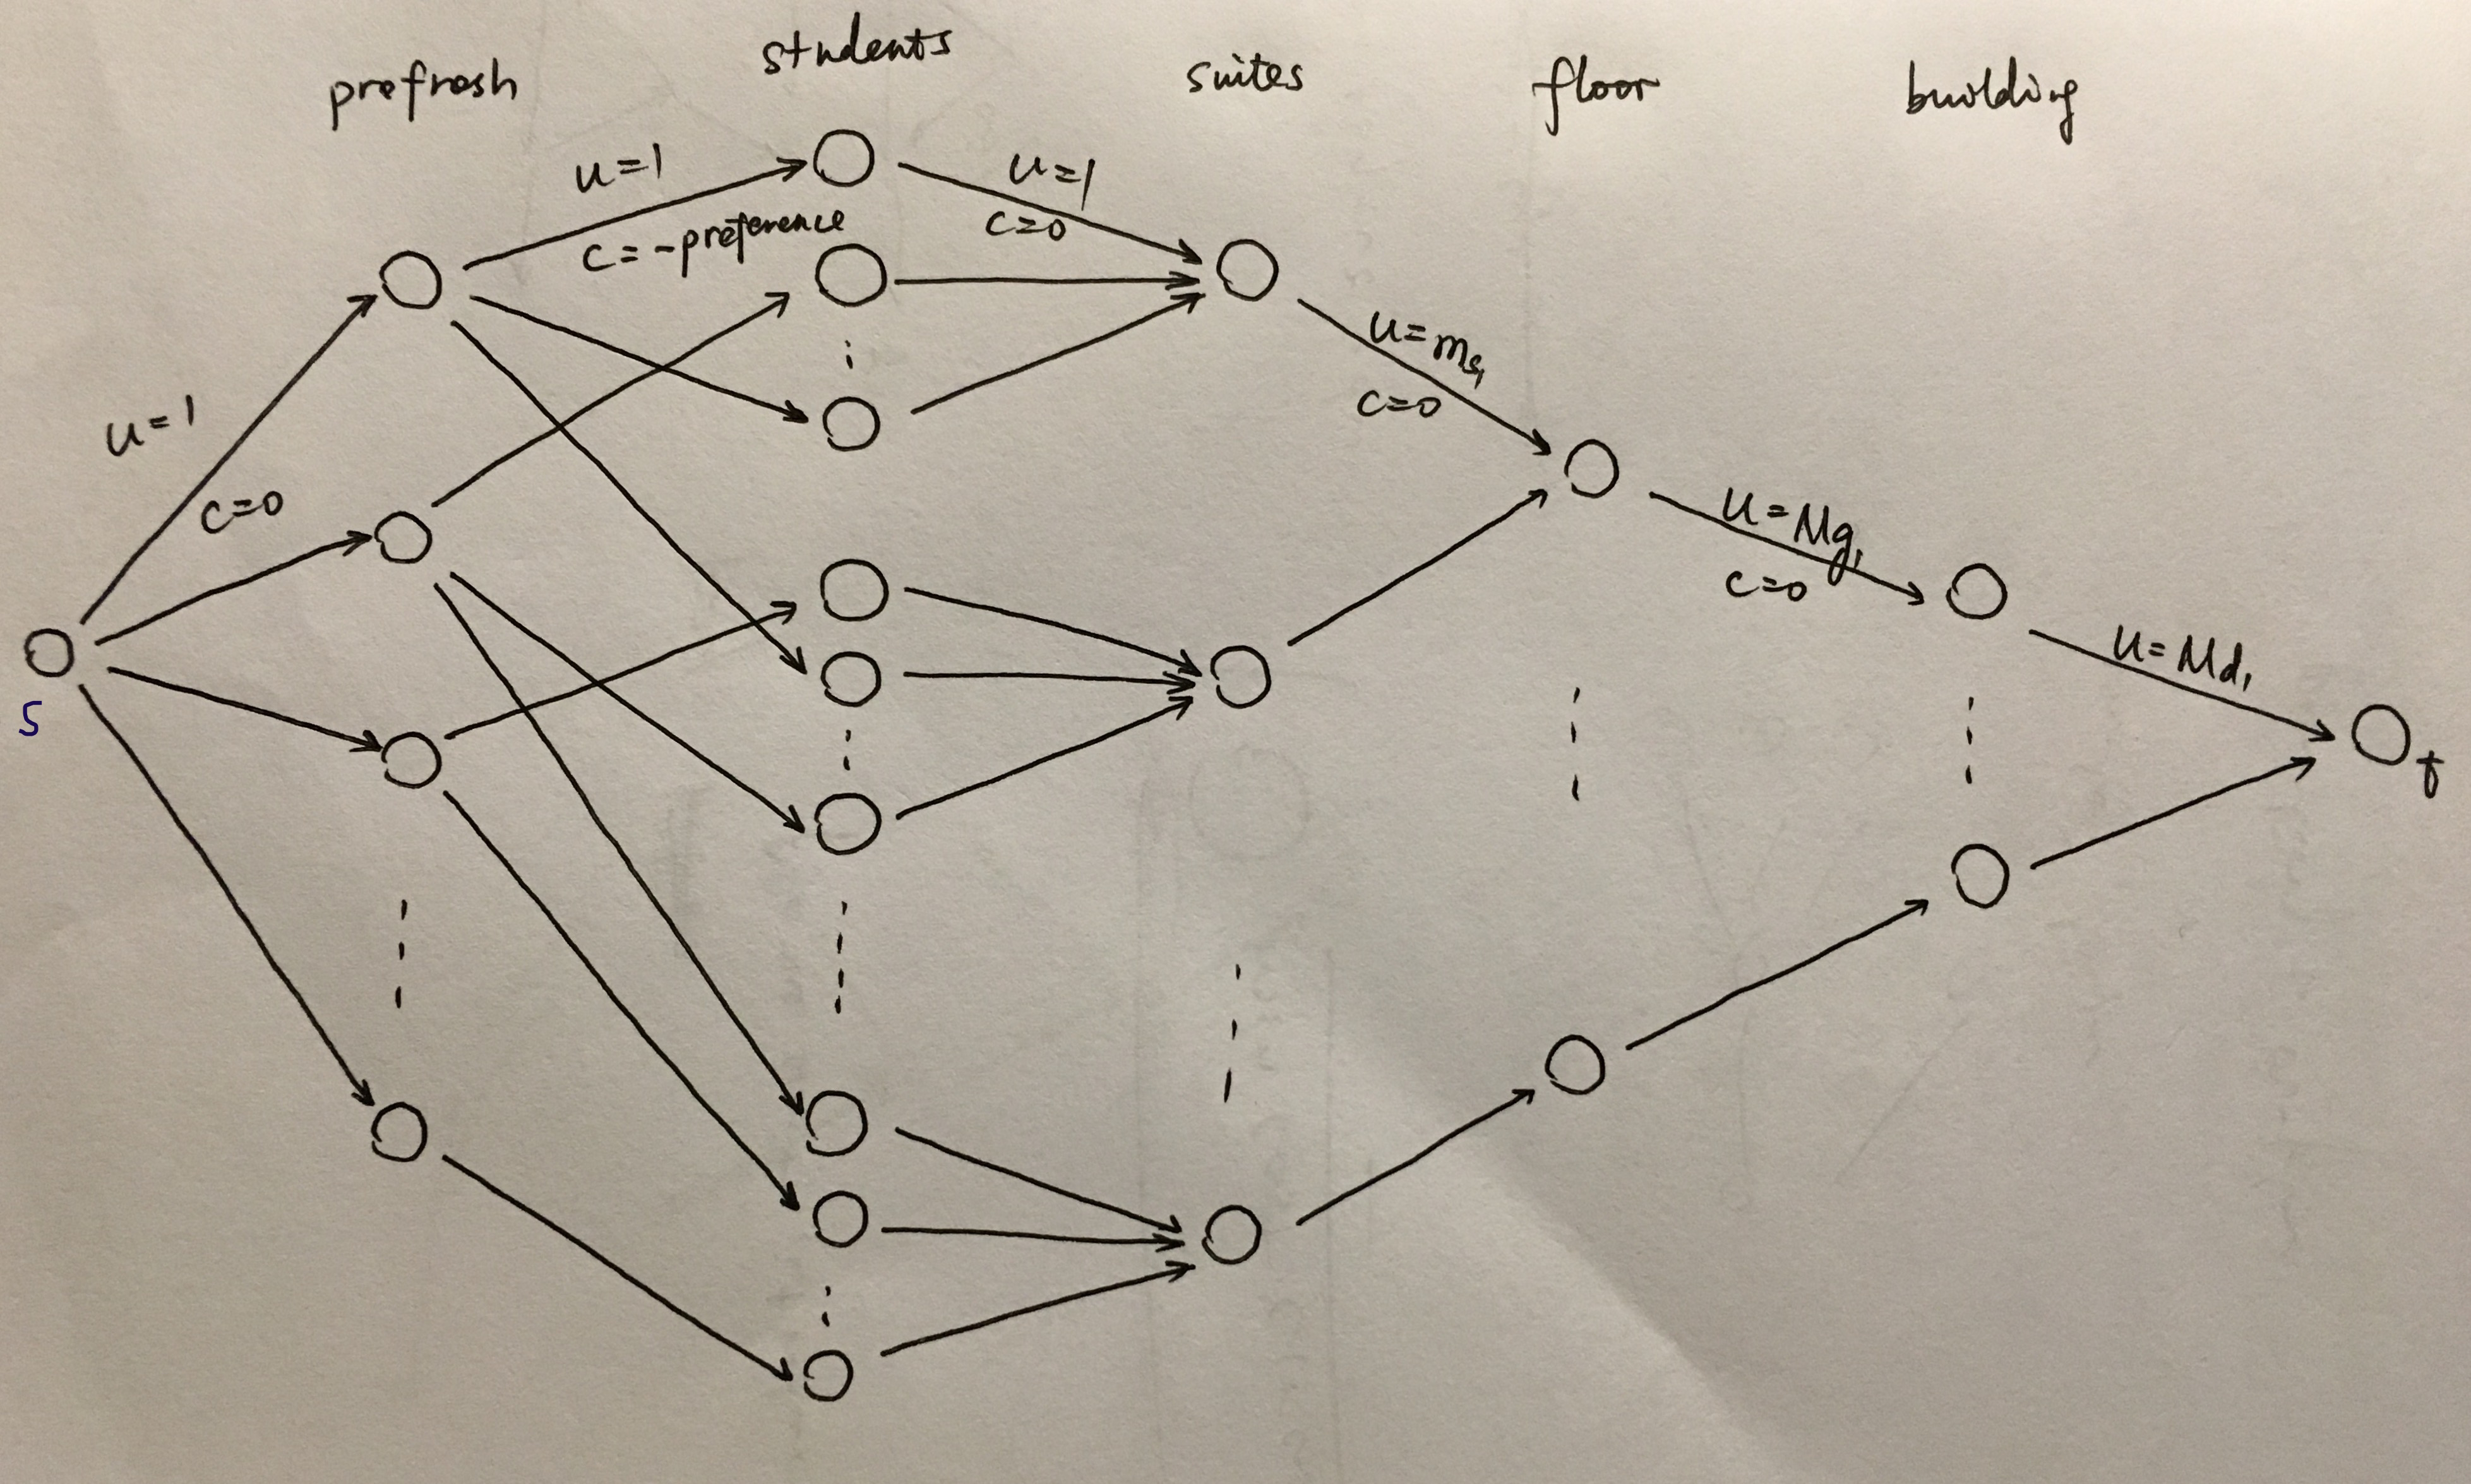
\includegraphics[width=1\textwidth]{5-a.jpg}
	\caption{Multi-layer graph for prefrosh assignment problem. The preference is encoded as the negative cost between prefrosh and students layer. No edge is assigned to those pairs with $-\infty$ preferences for simplicity. The capacity of suites is encoded in link capacity between suites and floor layer. The fire-codes for floors and dormitory are encoded in link capacity between floors and dormitory, and link capacity between dormitory and sink dormitory, respectively.}
	\label{fig:5-a}
\end{figure}
\paragraph{(b)} In order to address overallocation of suites, we introduce new `backup' suite nodes for each suite, shown as blue nodes in Figure \ref{fig:5-b}. Then we connect each student nodes that belong to the suite to the new suite node, with capacity $1$ and cost $0$. Next, connect the new suite node to the corresponding floor node, with capacity $+\infty$ and cost $-\sum_{all\:feasible\:prefrosh-student\:pair} preference$. All other nodes encoding the preferences and firecodes remain the same. 

Then, we run a min-cost max-flow algorithm as (a). If the total max-flow equals to the total number of prefrosh, i.e., all links from source are saturated, we have a feasible assignment. This is because now we can assign the prefrosh based on the flow values on the link. The firecodes are obeyed because the capacities on suite-floor floor-dormitory are unchanged. Notice that we overallocate a suite if the `backup' node has flow through, as the cost using the corresponding link is higher than all prefrosh-student links, it means there is no other way assigning prefrosh to students, which could have reduced the total cost. Also, as above, if there is a feasible solution, the algorithm is able to find it. Because otherwise we could have assigned the solution values to the link resulting in a max flow, which contradict with the fact that the algorithm returns a max flow. As a contrapositive statement, if the algorithm returns a max flow smaller than total prefrosh, there is no feasible solution to the problem.

The min-cost gives the most satisfying total preferences, even in the overallocation case. This is because the minimum of negative preference as costs maximizes the total preferences. In the overallocation case, notice that costs on the link connecting to the backup node are all the same, therefore it will not influence the `most satisfying' matching for prefrosh and students. 
\begin{figure}[h!]
	\centering
	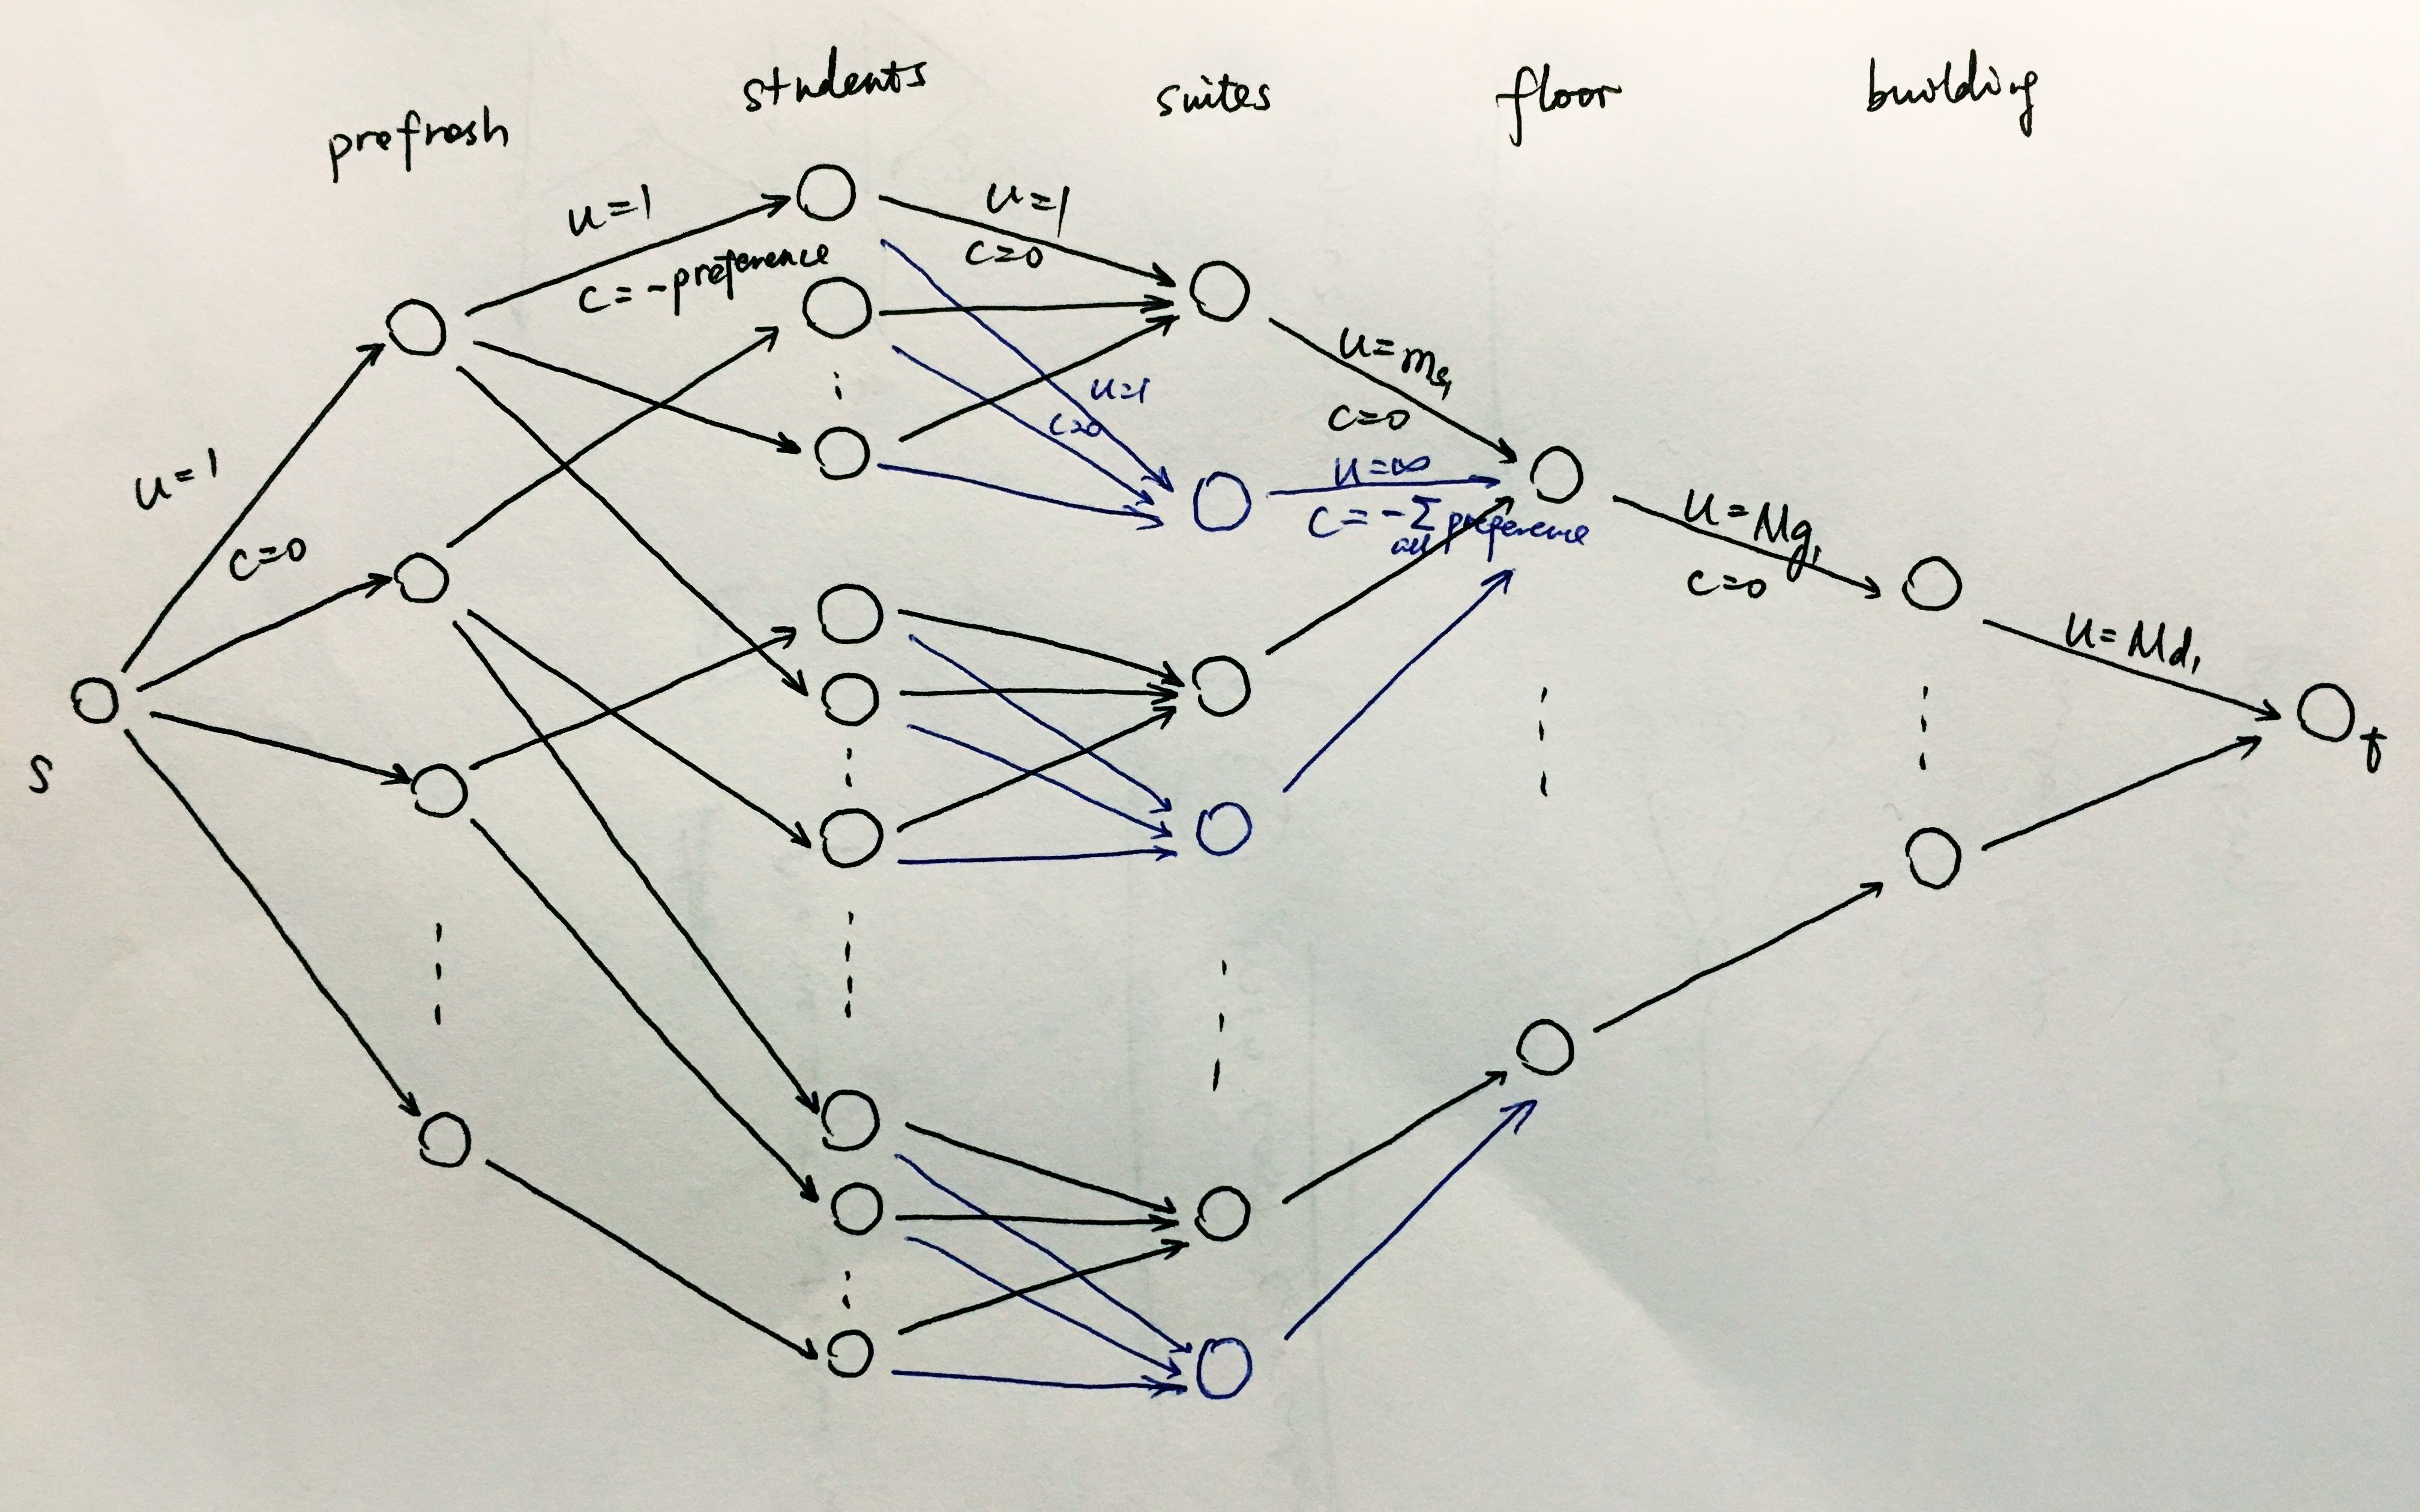
\includegraphics[width=1\textwidth]{5-b.jpg}
	\caption{Modified graph for overusing some suites. `Backup' nodes (blue) for each suites are added on the graph. Each new node is connected to students in the suite as before, but the link between backup suite nodes and floor node has cost $-\sum_{all\:paris}preferences$. The firecodes are still enforced in the link capacity of floor and dormitory as before.}
	\label{fig:5-b}
\end{figure}
\end{document}